\chapter{Implementation and code structure}
\label{code}
% \thispagestyle{empty}

\noindent 



\section{Overview}
We briefly explain here what kind of data are expected as input, the general workflow and the output of the software. In section \ref{c++}] more detailed implementation is discussed with focus on the R interface in section \ref{R} and the shared-memory parallelization in \ref{openmp}.

\subsection{Input data}
User provides a dataset of observations, each row a statistical unit, all belong to the same statistical model and have the same length. \\
Those are the data for our problem and they fulfil hypothesis of compositional data observation, e.g. sum constraint. Using the histogram example, each row consist of a histogram and all the histograms come from the same underlying model, e.g. proportion of annual income aggregated in classes for different region of a given country as in \cite{paper:pacs}. The values of a given row correspond to the "height" of each class of the histogram

User provides also what in splines lexicon are called the \textit{control points}, i.e. the middle point abscissa of each class of the histogram. Those abscissa are the same for all the rows of the dataset.

Strictly related to the optimal smoothing problem, spline degree \textit{k}, penalization order \textit{l}, smoothness tuning parameter \textit{$\alpha$} and spline knots must be provided. Spline knots can be passed as a given vector or they can be builded by default equispaced given the size.
\subsection{Count zeros: the Bayesian-multiplicative treatment} \label{BM}
In order to perform the clr map we have to compute a logarithm, so we have to ensure that all data are strictly positive. But some observation could be zero for different reason, in this framework we consider just the count-zero case using the lexicon of \cite{fernandez:zeros}, i.e. unobserved positive values that may have been observed with a larger number of trials or with a different sampling design.

We decided to rely on the Bayesian-multiplicative (BM) treatment described in \cite{fernandez:zeros}, which basically use a conjugate Dirichlet model for the normalized observation with uniform prior:
\[ \bm{X} \sim Dir(D,s\bm{t}) \]
\[ \bm{t} \sim U(1/D) \]

where $D$ is the dimension and $s$ tunes the strength of the prior. Using different values for $s$, we distinguish different priors, in particular we let the user choose among the ones showed in table \ref{fig:priors}.

\begin{figure}[ht]
	
	
	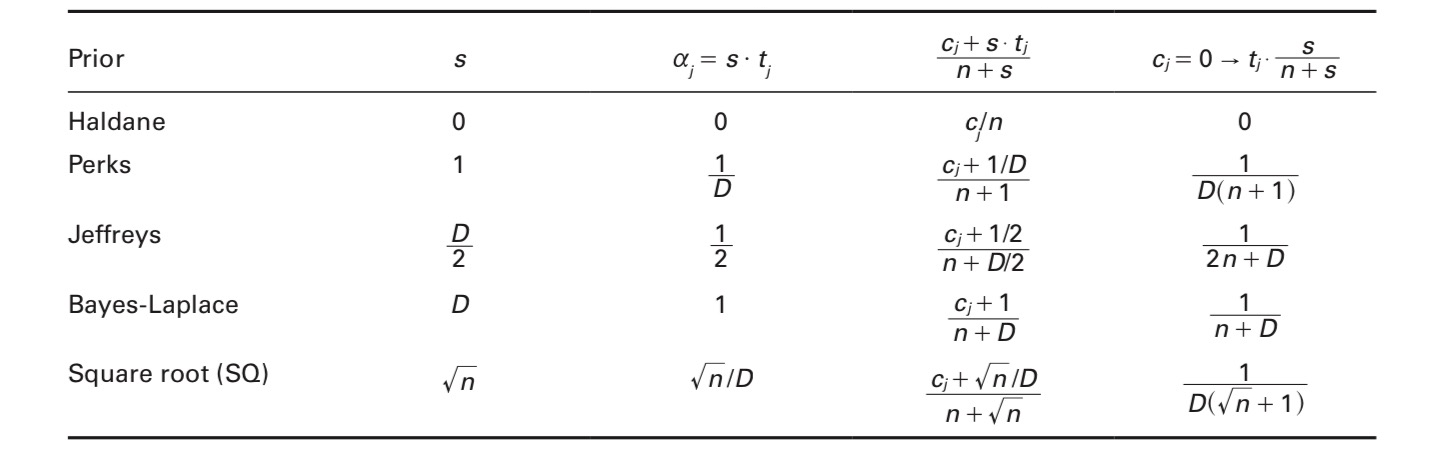
\includegraphics[width=\textwidth]{./pictures/BM/BMpriors.png}
	\label{fig:priors}
	
	\caption{BM priors (source \cite{fernandez:zeros}): $\bm{c}_{i}=(c_{i1},..,c_{iD})$ is the observed vector with some count-zeros, while $n_{i}=\sum_{j=1}^{D}c_{ij}$ is the total mass. Keep in mind that $t_{i}=1/D \quad \forall i$ since uniform priors are assumed.}
	\label{fig:priors}
	
\end{figure}

Finally the BM treatment ``corrects'' the count-zeros using the Bayesian posterior estimate. So if $\bm{c}_{i}=(c_{i1},..,c_{iD})$ is the observed vector with some count-zeros, defined $n_{i}=\sum_{j=1}^{D}c_{ij}$ the total mass, we use the posterior estimate formula on $\bm{x}_{i}=\bm{c}_{i}/n_{i}$, i.e. we replace $\bm{x}_{i}$ with $\bm{r}_{i}$ defined as:

\[ r_{ij} = 
\begin{cases} 
t_{ij} \, \frac{s_{i}}{n_{i}+s_{i}}, & \mbox{if } x_{ij}=0 \\ 
x_{ij}(1-\sum_{k:x_{ik}=0} \, t_{ik} \, \frac{s_{i}}{n_{i}+s_{i}}), & \mbox{if } x_{ij}>0 
\end{cases} \]

This has been implemented in the \verb|zeros| header and source files.

\subsection{Workflow} \label{workflow}
Parameters of the spline problem, including knots and control points, are stored in \verb|densityEstimator| class. This class contains all the fixed information of the problem, common to every row of the dataset to be processed. Through corresponding methods all the matrix requested to build the linear system described previously are computed and stored using \verb|Eigen| in such class.

\verb|dataManager| class deals with data. It reads a data-row, perform the zeros treatment and through the \verb|pacs| method solve the b-spline problem calling the \verb|solve| method of the \verb|densityEstimator| object. The result is written in a proper \verb|Eigen| structure. Using the \verb|plotData| method the resulting spline is finally evaluated in a given grid of point.

The reason of this structure of the code is due to the parallelization and it will be better understood in section \ref{openmp}.

\subsection{Output}
Output consist in b-spline coefficients for each statistical unit and possibly a grid of values in which resulting b-splines are evaluated at. \\ Size of the grid can be given as input parameter, otherwise it is handled by default.

\section{R/C++ interface} \label{R}
\subsection{\texttt{.Call} and \texttt{RcppEigen}}
Code structures, implementation choices and C++ programming style reflect the necessity to develop an efficient implementation of the discussed density estimation method together with the flexibility and the comfort of the R environment for further analysis. \\ All of that is done via the R package facility with our \verb|splineDensity| package available in the git repository (see section \ref{installation} for installation details). 

The interface used to execute C++ code in R is \verb|.Call| described in [cit]. Let us provide a simple example of how it works, this is our C++ example:

\begin{lstlisting}
#include <R.h>
#include <Rinternals.h>
extern "C"{
SEXP add(SEXP a, SEXP b) {
SEXP result = PROTECT(allocVector(REALSXP , 1)); REAL(result)[0] = asReal(a) + asReal(b); UNPROTECT (1);
return result;
} }
\end{lstlisting}

and this is what we run in R:

\begin{lstlisting}
dyn.load("mysharedlib.so")
add <- function(a, b) { .Call("add", a, b)
}
\end{lstlisting}

After we compile our C++ code in a dynamic library via command line with \verb|R CMD SHLIB| or using the compiler directly, we can load the library in the R environment using \verb|dyn.oad()|. After our object is loaded we can directly use the C++ function with \verb|.Call("add",a,b)|, e.g. defining an R function named "add".

In the C++ code all kind of object that come from R or should be return to R are of the \verb|SEXP| type. The power of this interface is that all R variables are not passed by copy, but by a particular kind of pointer (the \verb|SEXP| type). As a consequence, to prevent that R garbage collection destroys objects which should be returned, it is important to use the \verb|PROTECT()| function. Finally all the code that R should be able to use (e.g. the defined function) must be included in the \verb|extern "C"| scope. \verb|SEXP| object can be copied in C++ objects through some specific functions defined in the R header files as \verb|REAL()| or \verb|INTEGER()|. 
 
\medskip

We decided also to rely on \emph{Rcpp}/\emph{RcppEigen} libraries [cit] which easily allow to interface R matrixes with \verb|Eigen| structures combining the \verb|Eigen::Map| method with the \verb|Rcpp::as| function, e.g.:

\begin{lstlisting}
SEXP Rmatrix;
Eigen::Map<Eigen::MatrixXd>  newMatrix(as<Eigen::Map<Eigen::MatrixXd>> (Rmatrix));
\end{lstlisting}

Note that this leads to have a complex type for the \verb|newMatrix| object, working with a row of it you have to consider the following type:

\begin{lstlisting}
Eigen::Block<Eigen::Map<Eigen::Matrix<double, -1, -1>,0, Eigen::Stride<0, 0> >, 1, -1, false>
\end{lstlisting}

\subsection{Debug}
It could happen that R session crashes due to some memory leakage, in such cases it could be hard to find the problem since the lack of reports from the R session. We have find really helpful the debug mode, which can be started with the following command from the terminal:

\begin{lstlisting}
R -d <debugger>
\end{lstlisting}

where \verb|-d| stays for "debug". In particular we relied a lot on the famous memory error detector \emph{valgrind} and we found it really useful.

\section{C++ implementation} \label{c++}

\subsection{\texttt{parametersManager}, \texttt{dataManager} and \texttt{densityEstimator} classes}

\begin{itemize}
\item \verb|parametersManager|: it includes problem parameters shared among all statistical units such as control points, knots, spline degree, penalization order and $\alpha$ value. No objects of this class are actually declared, but it is conceptually useful to distinguish it from its child \verb|densityEstimator|.

\item \verb|densityEstimator|: it inherits publicly from \verb|parametersManager|. It has methods to compute all the necessary matrixes and the final linear system described in \ref{optimal}. it has a method to evaluate the J functional and the \verb|solve| method which is described in \ref{solvemethod}. Such method is used on each row (parameters and problem matrix are common) and return the estimated b-spline coefficients.

\item \verb|dataManager|: it used to interface the data with the smoothing process. It reads a row of the data set and then performs the BM treatment (section \ref{BM}). The \verb|pacs| method has the \verb|densityEstimator| object as argument and calls the \verb|solve| method saving the output (spline coefficients) in a given matrix. It has also methods to evaluate the estimated function in a grid of points both in the clr space and the reference space, respectively \verb|plotData| and \verb|plotData_Clr| methods.

\begin{figure}[ht]
	
	
	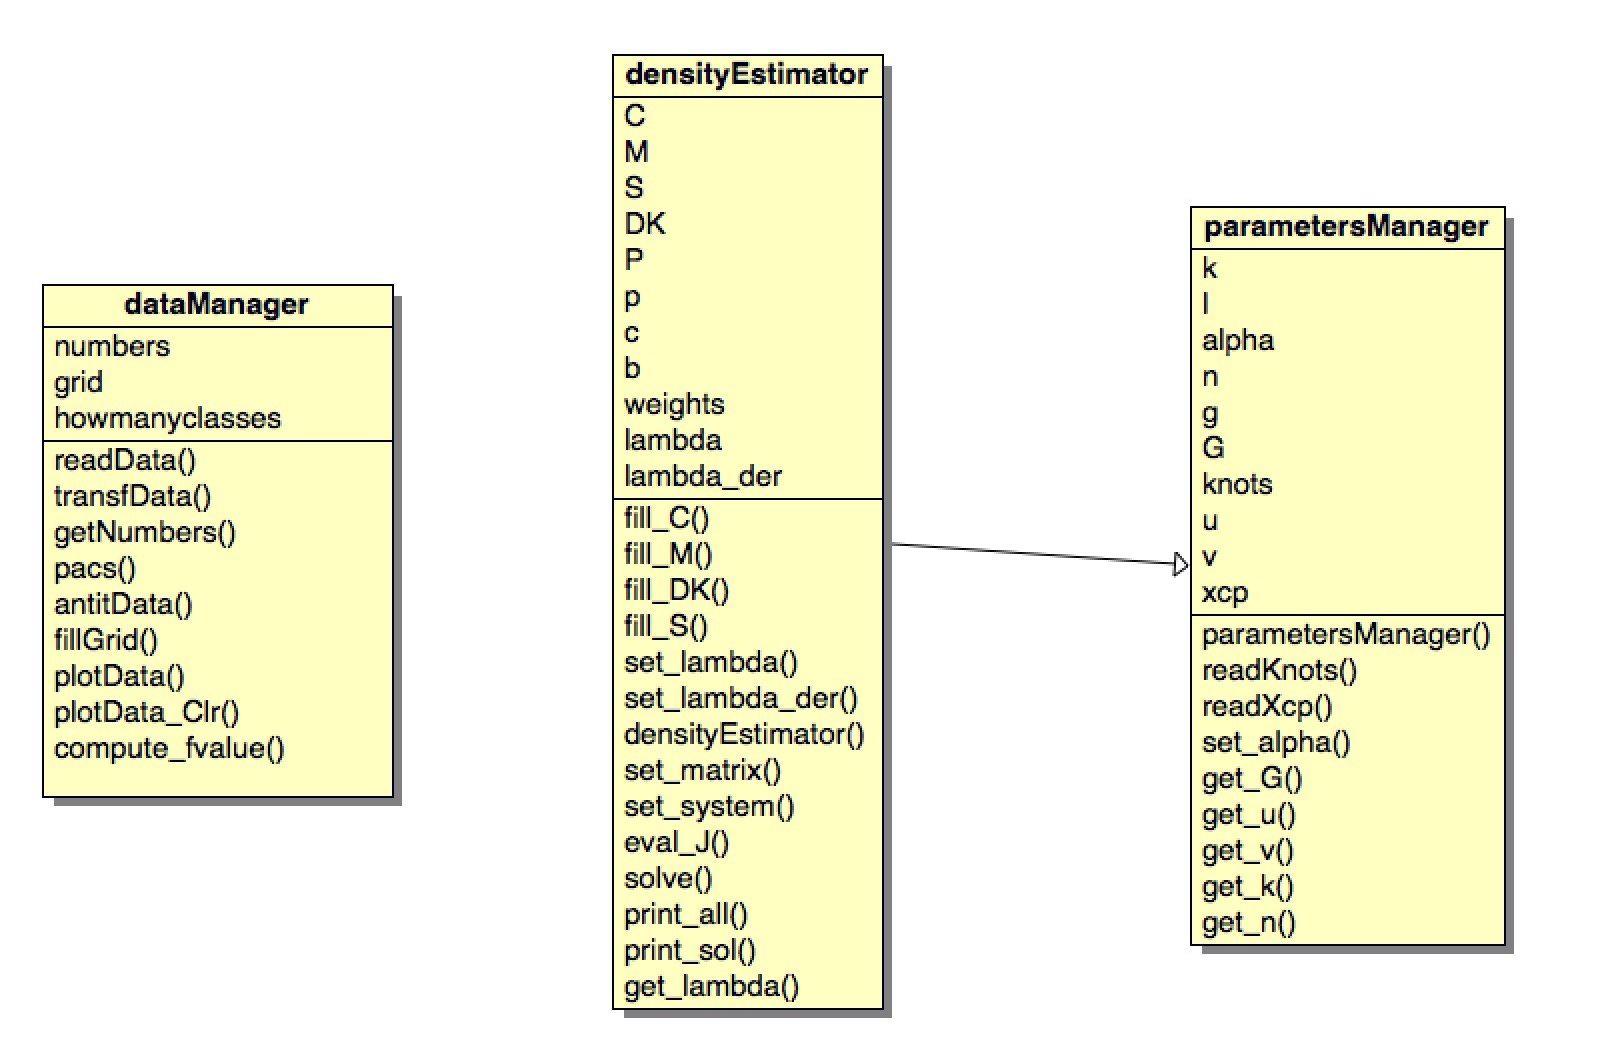
\includegraphics[width=\textwidth]{./pictures/classes/class_diagram.jpg}
	\label{fig:diagram}

	\caption{Classes diagram}
	\label{fig:diagram}
	
\end{figure}

\end{itemize}

\subsection{Solve method} \label{solvemethod}
As already discussed in section \ref{optimal}, the smoothing problem could not have a solution, in such case a minimum norm solution should be provided.
We decided to rely on the \verb|FullPivHouseholderQR| solver provided by the \verb|Eigen| library, which apply Householder rank-revealing QR decomposition with full pivoting. This decomposition performs a very prudent full pivoting in order to be rank-revealing and achieve optimal numerical stability. 

Rank-revealing property is very important in case we want to find a solution when the problem is not solvable. Kernel knowledge allows us to analytically find a minimum norm solution in case its dimension is 1 or 2:

\[ A\bm{x}=\bm{b} \]

If dim(Ker($A$))$=1$,
	
\[ \bm{k}\in\text{Ker{A}} \quad \text{and} \quad \bm{\hat{x}} \quad \text{found solution} \]
\[ c=\frac{<\bm{\hat{x}},\bm{k}>}{<\bm{k},\bm{k}>} \]
\[ \bm{x}_{\text{min}} = \bm{\hat{x}} - c\bm{k} \]
else if dim(Ker($A$))$=2$, let
\[ \bm{k_1}, \bm{k_2} \in\text{Ker{A}} \quad \text{and} \quad \bm{\hat{x}} \quad \text{found solution,} \]
then, doing elementary computations,
\begin{align*}
\left( \| \bm{k_2} \|^2 - \frac{<\bm{k_1},\bm{k_2}>^2}{<\bm{k_1},\bm{k_1}>} \right) &c_2 = \, <\bm{\hat{x}},\bm{k_2} - \frac{<\bm{k_1},\bm{k_2}>}{<\bm{k_1},\bm{k_1}>} \, \bm{k_1}> \\
&c_1 = - \frac{<\bm{k_1},\bm{k_2}>}{<\bm{k_1},\bm{k_1}>} \, c_2 +  \frac{<\bm{\hat{x}},\bm{k_1}>}{<\bm{k_1},\bm{k_1}>}
\end{align*}  
\[ \bm{x}_{\text{min}} = \bm{\hat{x}} - c_1\bm{k_1} - c_2\bm{k_2} \]


Otherwise, when kernel dimension is greater than 2 we decided to apply Tychonoff regularization ($\lambda=0.01$) to the matrix problem in order to achieve full rank and find a solution. Obviously in such case we will be solving an approximation of our problem:

\[  \hat{A}=A + \lambda I \]
\[  \text{new problem} \quad \hat{A}\bm{x}=\bm{b} \]

All that is done by the \verb|solve| method of the \verb|densityEstimator| object through a \verb|switch| statement over the kernel dimension.

\subsection{Cross-validation function} \label{cv}
In addition to the resolution of the optimal problem, we were asked to provide a cross-validation method to asses the best $\alpha$ among a vector of choices. Such validation has been designed to be a sort of leave-one-out (LOO) algorithm: one at a time each control point (c.p.), which is not an extremal, is left out, the b-spline is estimated and the error is computed as the sum of the differences between the left out values and the corresponding estimate given by the b-spline averaged among all the rows:

\[ \forall \alpha_{i}\in\bm{\alpha}  \quad \text{error}_{LOO}(\alpha_{i}) = \sum_{k=1}^{\#rows}\sum_{j=1}^{\#c.p.} \frac{\\| y_{k,j}-\hat{y}_{k,j} \\| }{\text{\#rows}} \]

After that the best $\alpha$ value is found and cross-validation errors among with evaluation of the J functional of the minimization problem are returned to the user, with best choice highlighted.

\section{OpenMP parallelization} \label{openmp}
In section \ref{workflow} was mentioned the fact that we perform the same operation over each row of the given data set in a \verb|for| loop. Precisely the matrix associated to the linear system is fixed and what changes is the constant term, which depends on the data. So after constructing the problem matrix, we loop over the row in the following way:

\begin{lstlisting}
for(std::size_t i = 0; i < nrow; i++)
{
  obj.readData(data.row(i), prior);
  obj.transfData();
  obj.pacs(dens,bsplineMat.row(i));
  obj.plotData(dens, numPoints, bsplineMat.row(i), yvalueMat.row(i));
  obj.plotData_Clr(dens, numPoints, bsplineMat.row(i), yvalueMatClr.row(i));
}
\end{lstlisting}

where \verb|obj| is a \verb|dataManager| object and \verb|dens| a \verb|densityEstimator| object.

This commands are easily parallelizable in shared memory framework as OpenMP, it is enough to ask each thread to solve the problem for a subset of rows. OpenMP gives also the possibility to make same objects private to each thread through the \verb|private| keyword. If those objects exists before the \verb|#pragma| statement then the \verb|firstprivate| keyword should be used to initialize them with their values. In a simple way the previous code become the following:

\begin{lstlisting}
@ \textcolor{magenta}{\#pragma omp parallel private(obj) firstprivate(dens)} @
  {
@ \textcolor{magenta}{\#pragma omp for} @
    for(std::size_t i = 0; i < nrow; i++)
    {
      obj.readData(data.row(i), prior);
      obj.transfData();
      obj.pacs(dens, bsplineMat.row(i));
      obj.plotData(dens, numPoints, bsplineMat.row(i), yvalueMat.row(i));
      obj.plotData_Clr(dens, numPoints, bsplineMat.row(i), yvalueMatClr.row(i));
   }
 }
\end{lstlisting}

Thanks to this multithreads implementation we achieved a satisfactory speed-up in the computations when a large data set is provided.

We tested the code on a dataset of $10^{6}$ rows and 12 column on a 12 cores Intel(R) Core(TM) i7-3930K CPU @ 3.20GHz machine, leaving out one core dedicated to the OS. Results are shown in figure \ref{fig:giuspo12}.

\begin{figure}[ht]
	
	\begin{subfigure}{.5\textwidth}
		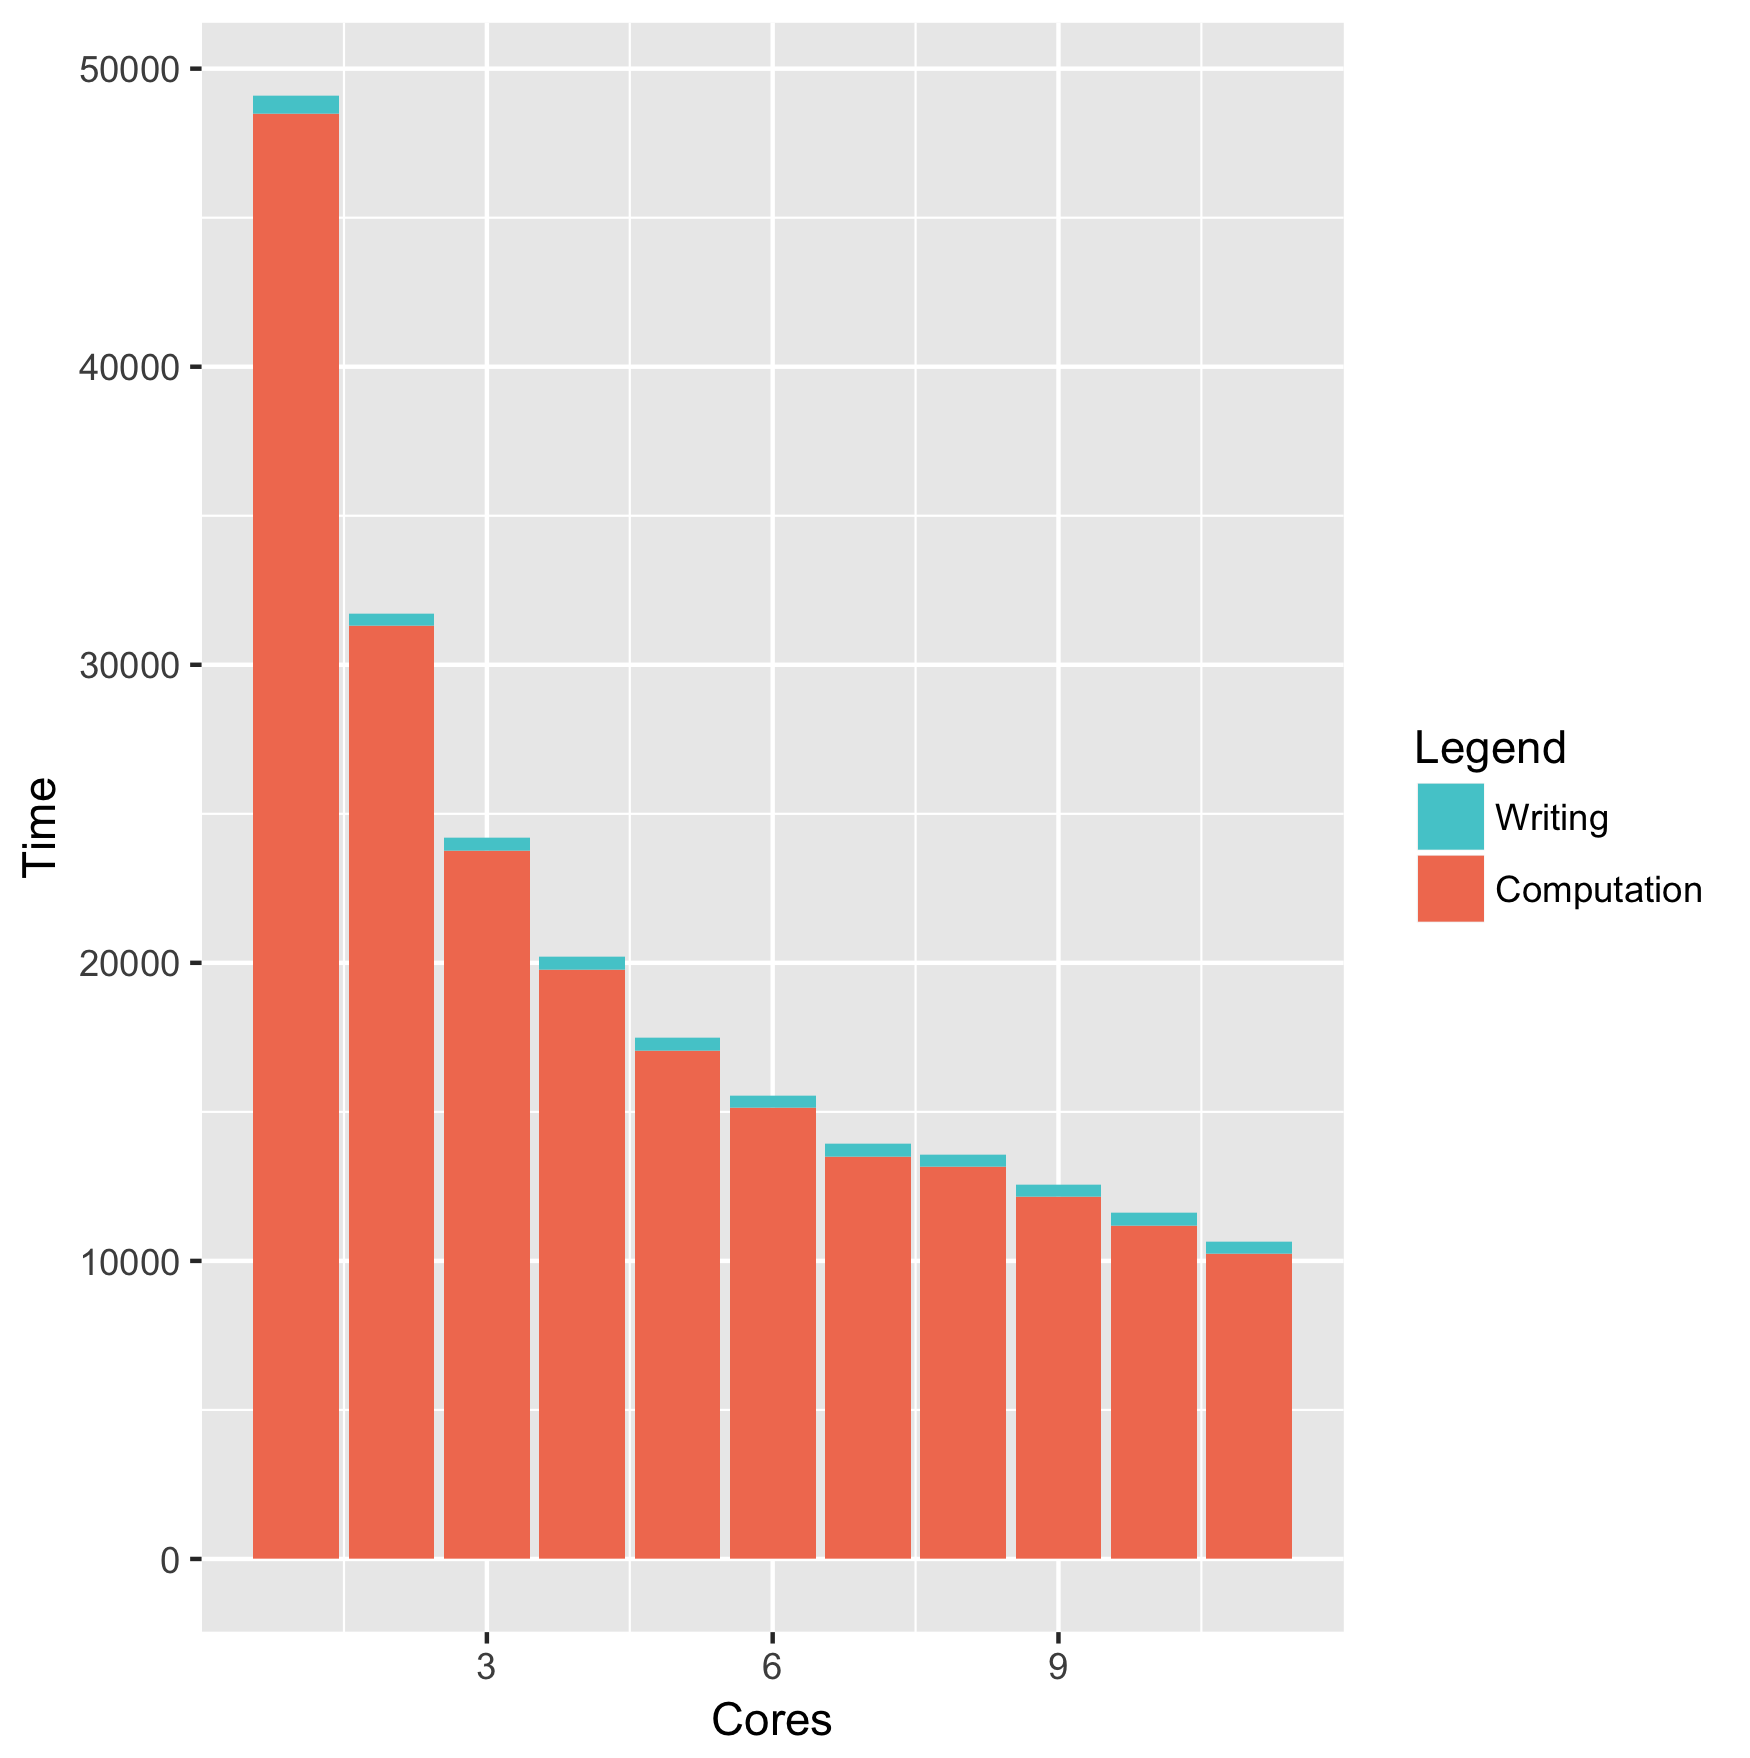
\includegraphics[width=6cm]{./pictures/openmp/giuspo12_time.png} 
		\label{fig:subim1}
	\end{subfigure}
	\begin{subfigure}{.5\textwidth}
		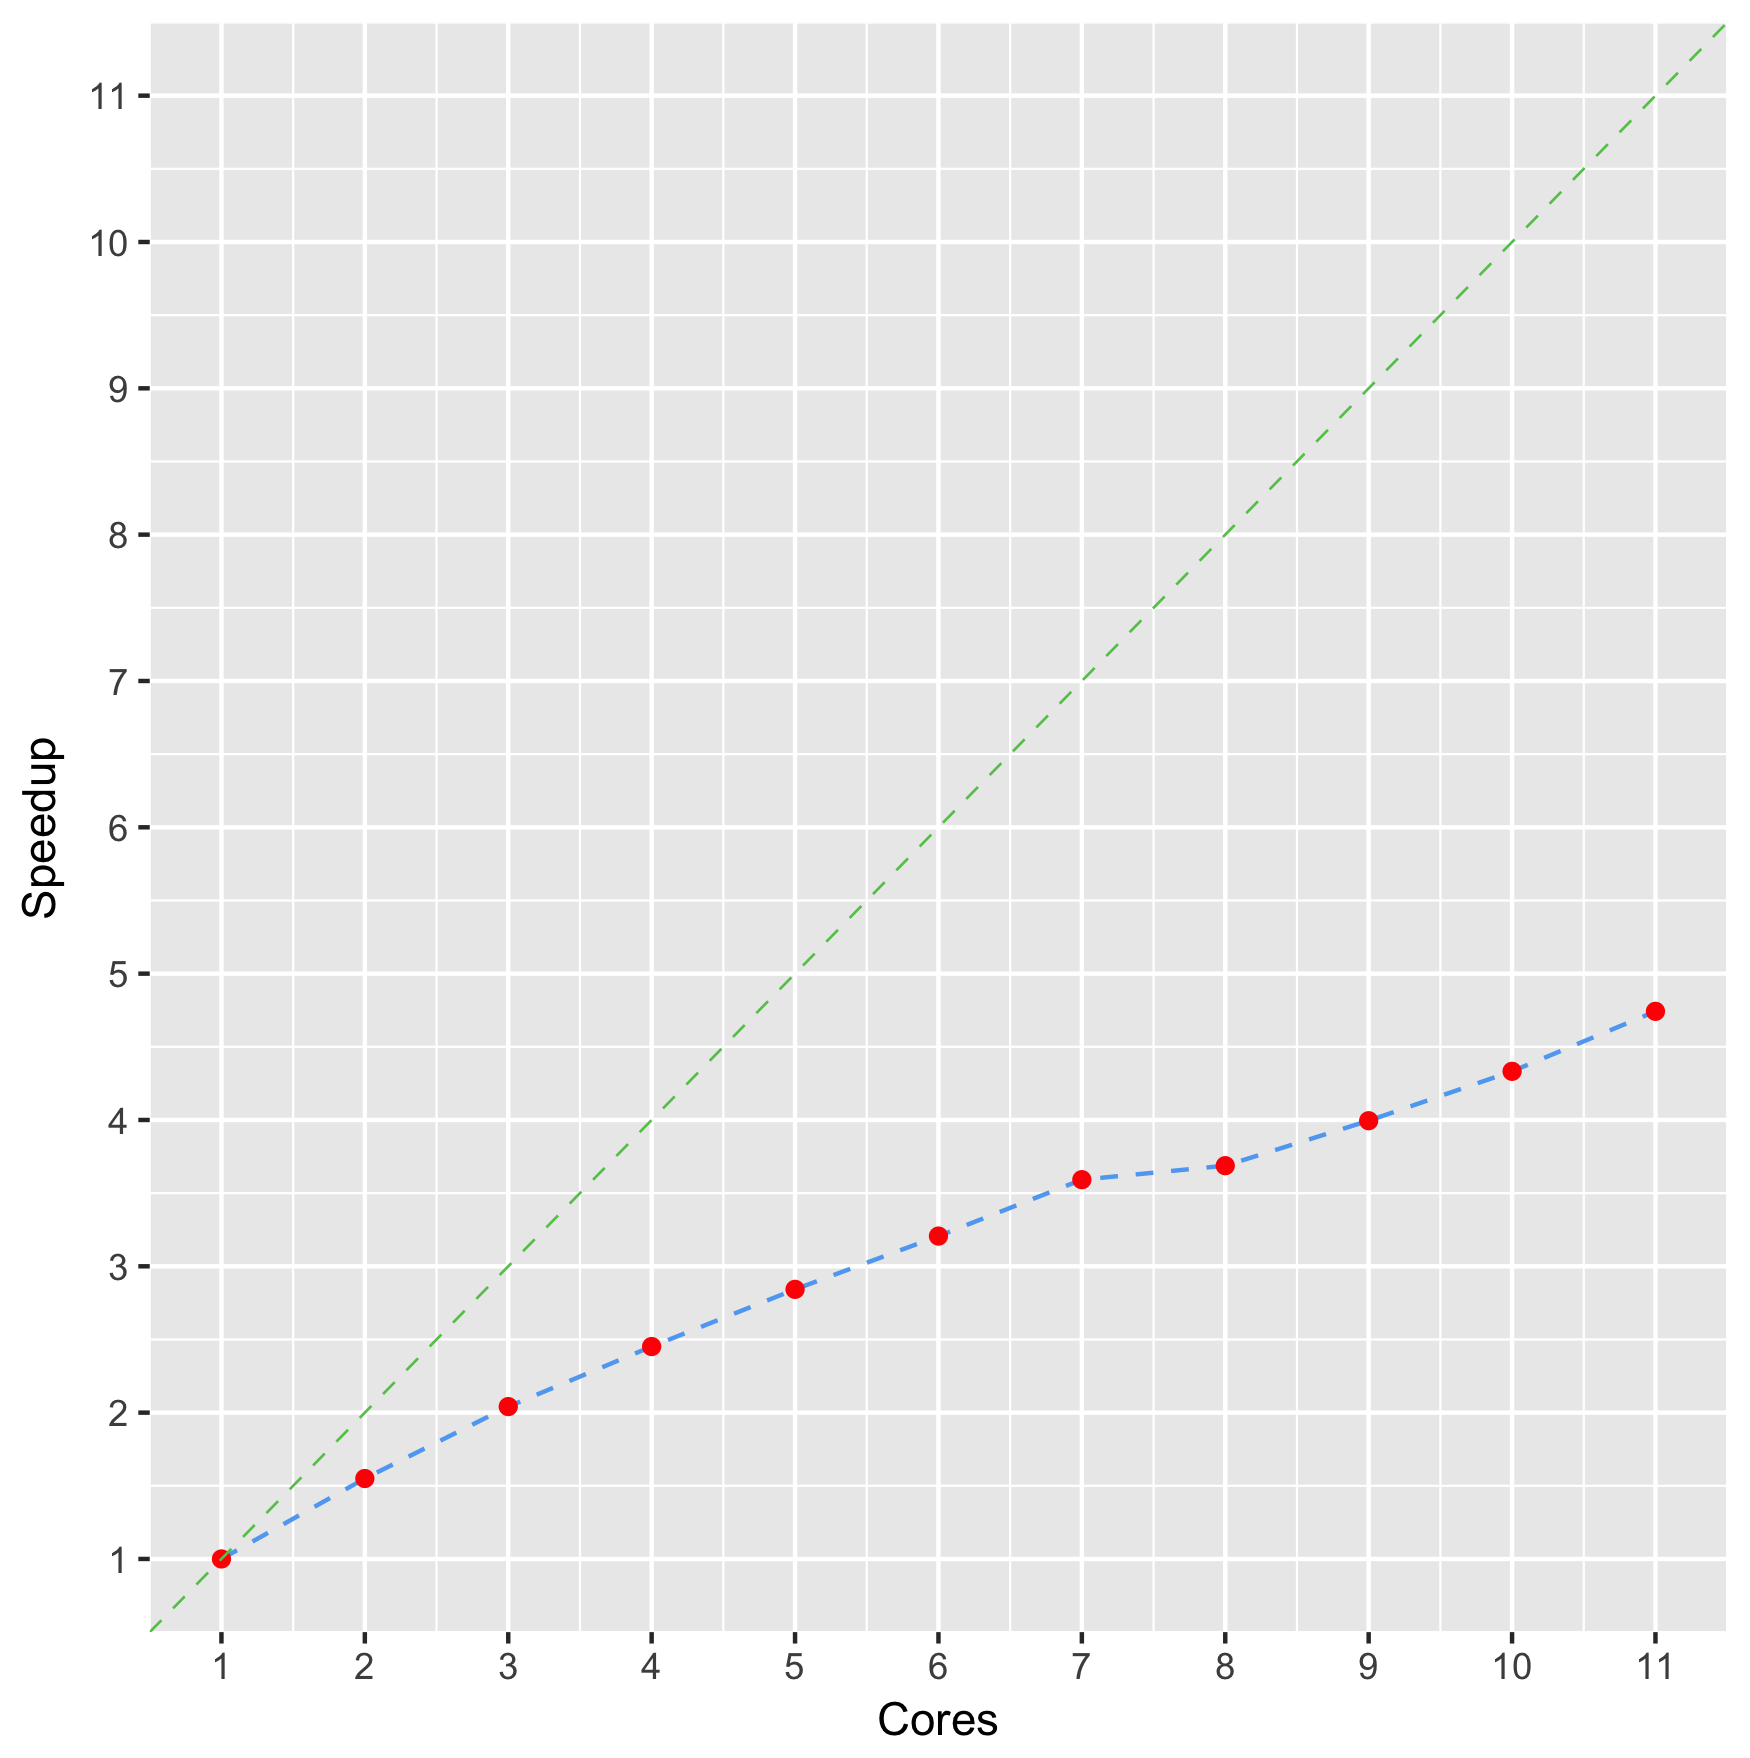
\includegraphics[width=6cm]{./pictures/openmp/giuspo12_speedup.png}
		\label{fig:subim2}
	\end{subfigure}
	
	\caption{Intel(R) i7-3930K CPU @ 3.20GHz: on the left time (milliseconds) required by the software divided in computation time (solve the problem) and writing time (write the solution in R objects, this is done by just one thread). On the right speed-up plot.}
	\label{fig:giuspo12}
	
\end{figure}


Cross-validation function (section \ref{cv}) has been parallelized over the different $\alpha$ values:

\begin{lstlisting}
@ \textcolor{magenta}{\#pragma omp parallel private(obj) firstprivate(dens)} @
  {
    Eigen::MatrixXd threadBsplineMat(nrow,dens.get_G());
    Eigen::ArrayXd N;
    int span;
    long double fvalue;

    @ \textcolor{magenta}{\#pragma omp for} @
    for(std::size_t z = 0; z < alpha_size; z++)
    {
      dens.set_alpha(alpha[z]);
      for(std::size_t i = 0; i < nrow; i++)
      {
        for(std::size_t j = 1; j < ncol-1; j++) 
        {
          // LOO-CV, leave out column j, fit spline and compute error
          dens.readXcp(Xcp,Xcpsize,j);
          dens.set_matrix();
          dens.set_system();
          obj.readData(data.row(i),prior,j);
          obj.transfData();
          obj.pacs(dens, threadBsplineMat.row(i));
          Jvalues(z)+=dens.eval_J(obj.getNumbers())/nrow;

          // computing error using spline coefficients, fvalue is the predicted value
          // [...]
        }
      }
    }
  }
  \end{lstlisting}

This time it was necessary to reserve each thread an \verb|Eigen| matrix (\verb|threadBsplineMat|) where to store the result of its partial computation. Note that every object defined inside the \verb|#pragma omp| statement is automatically private to each thread. Comparison to asses the best $\alpha$ value is done outside the parallelized scope by one single thread.




% struttura generale del codice: cosa in input, cosa in output
% scelta di salvare le matrici con eigen sparse, dimensione matrici
% problema zero-forcing
% densityEstimator figlia di parametersManager (che � "astratta")